\documentclass{article}
\usepackage{fontspec}
\usepackage{type1cm}
\usepackage{graphicx}
\usepackage{geometry}
\usepackage[bold-style=ISO]{unicode-math}
\usepackage[heading=true]{ctex}%添加heading=true,使用中文版式
\geometry{a4paper,left=1cm,right=1cm,top=3cm,bottom=3cm}
\usepackage{titlesec} %自定义多级标题格式的宏包
\titleformat{\section}[block]{\Huge\bfseries}{\arabic{section}}{1em}{}[]
\titleformat{\subsection}[block]{\huge\bfseries}{\arabic{section}.\arabic{subsection}}{1em}{}[]
\titleformat{\paragraph}[block]{\LARGE\bfseries}{[\arabic{paragraph}]}{1em}{}[]

\begin{document}
\begin{flushleft}
	\LARGE
	% \qquad 缩进两个字符
	
	\section{公式}

	\subsection{二维邻域}
	以点$P_0(x_0,y_0)$为圆心,$\delta$为半径围成一个圆。圆内所有的点(不包括圆的边)的集合称为$P_0$的$\delta$邻域,记为$U(P_0,\delta)$\\
	
	\subsection{二元函数}
	二元函数$z=f(x,y)$的图像在三维坐标里是曲面\\
	二元函数的可导与连续无关\\
	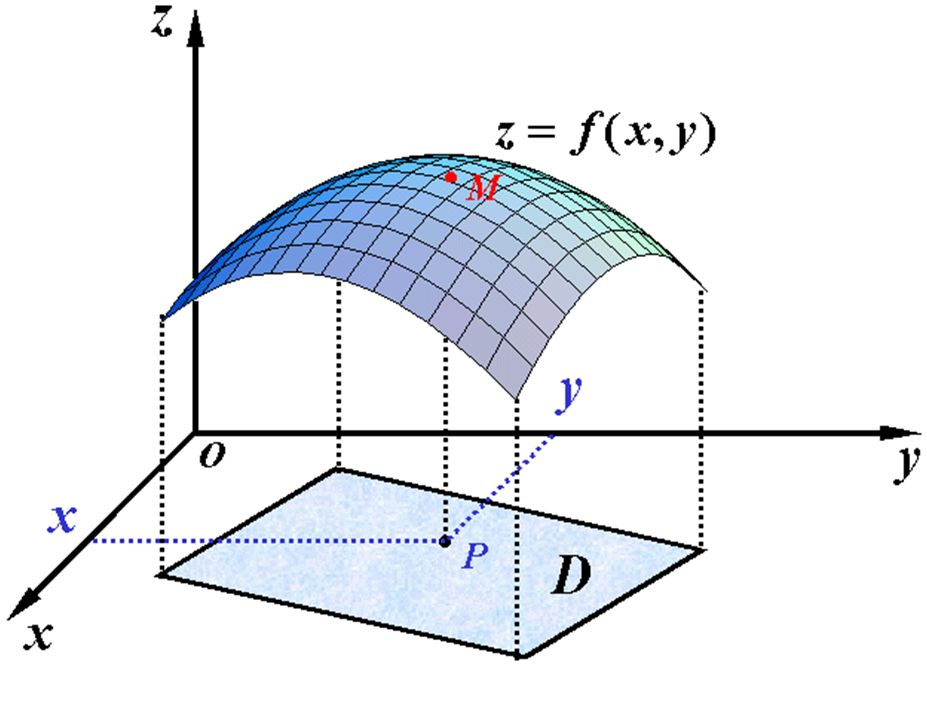
\includegraphics[scale=0.5]{eyhstx.jpg}
	
	\subsection{二元函数的极限}
	$\lim\limits_{\substack{x\to x_0\\ y\to y_0}}f(x,y)=A$\\
	注意:二元函数求极限不能使用洛必达法则和单调有界准则\\
	~\\
	若$\lim\limits_{\substack{x\to x_0\\ y\to y_0}}f(x,y)=f(x_0,y_0)$,则$f(x,y)$在点$(x_0,y_0)$连续\\
	
	\subsection{偏导数}
	\paragraph{偏导数的定义}
	$f_x'(x_0,y_0)=\lim\limits_{x\to x_0}\frac{f(x,y_0)-f(x_0,y_0)}{x-x_0}$\\
	$f_y'(x_0,y_0)=\lim\limits_{y\to y_0}\frac{f(x_0,y)-f(x_0,y_0)}{y-y_0}$\\
	
	\paragraph{求偏导数}
	1、对$x$求偏导:将$y$看作常数后再对$x$求导\\
	2、对$y$求偏导:将$x$看作常数后再对$y$求导\\
	
	\paragraph{偏导数的几何意义}
	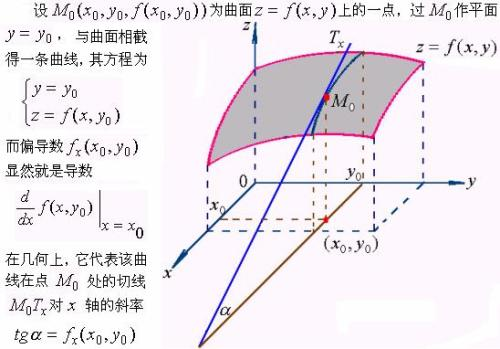
\includegraphics[scale=1.0]{pdsjhyy.jpg}
	
	\subsection{二阶偏导数}
	
	\paragraph{按照对变量的求导顺序不同,二阶偏导数有以下四个}
	1、$\frac{\partial}{\partial x}(\frac{\partial z}{\partial x})=
	\frac{\partial^2z}{\partial x^2}=f_{xx}''(x,y)$\\
	2、$\frac{\partial}{\partial y}(\frac{\partial z}{\partial x})=
	\frac{\partial^2z}{\partial x\partial y}=f_{xy}''(x,y)$\\
	3、$\frac{\partial}{\partial x}(\frac{\partial z}{\partial y})=
	\frac{\partial^2z}{\partial y\partial x}=f_{yx}''(x,y)$\\
	4、$\frac{\partial}{\partial y}(\frac{\partial z}{\partial y})=
	\frac{\partial^2z}{\partial y^2}=f_{yy}''(x,y)$\\
	~\\
	其中$\frac{\partial^2z}{\partial x\partial y}$和$\frac{\partial^2z}{\partial y\partial x}$称为混合偏导数\\
	
	\paragraph{定理}
	若$z=f(x,y)$的两个二阶混合偏导数$\frac{\partial^2z}{\partial x\partial y}$和
	$\frac{\partial^2z}{\partial y\partial x}$在点$(x_0,y_0)$处连续,
	则$\frac{\partial^2z}{\partial x\partial y}|_{(x_0,y_0)}=
	\frac{\partial^2z}{\partial y\partial x}|_{(x_0,y_0)}$\\
	
	\subsection{全微分}
	
	设$z=f(x,y)$,若全增量$\Delta z=f(x_0+\Delta x,y_0+\Delta y)-f(x_0,y_0)$可表示为$\Delta z=A\Delta x+B\Delta y+o(\rho)$,其中$\rho=\sqrt{(\Delta x)^2+(\Delta y)^2}$,则称$z$在$(x_0,y_0)$处可微\\
	$A\Delta x+B\Delta y$称为$z$在$(x_0,y_0)$处的微分,记为$dz|_{(x_0,y_0)}=A\Delta x+B\Delta y$,
	且$\lim\limits_{\substack{\Delta x\to 0\\ \Delta y\to 0}}\frac{\Delta z-(A\Delta x+B\Delta y)}{\sqrt{(\Delta x)^2+(\Delta y)^2}}=0$\\
	~\\
	若$z=f(x,y)$在点$(x_0,y_0)$处可微,则$f(x,y)$在点$(x_0,y_0)$处连续且可偏导,且微分$dz=\frac{\partial f}{\partial x}|_(x_0,y_0)dx+\frac{\partial f}{\partial y}|_(x_0,y_0)dy$\\
	~\\
	若$z=f(x,y)$的两个偏导数$\frac{\partial f}{\partial x}$和$\frac{\partial f}{\partial y}$都在点$(x_0,y_0)$处连续,则$z=f(x,y)$在点$(x_0,y_0)$处可微\\
	
	\subsection{多元复合函数求偏导}
	
	1、将函数$z=f(u(x,y),v(x,y))$画成如下的关系图:\\
	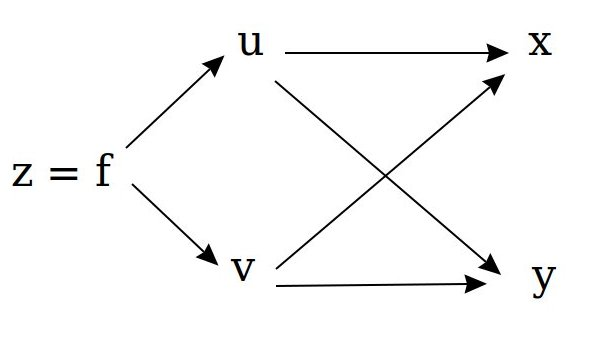
\includegraphics[scale=0.5]{lsqdfz.jpg}\\
	2、$\frac{\partial z}{\partial x}=\frac{\partial f}{\partial u}\cdot\frac{\partial u}{\partial x}+\frac{\partial f}{\partial v}\cdot\frac{\partial v}{\partial x}$\\
	3、$\frac{\partial z}{\partial y}=\frac{\partial f}{\partial u}\cdot\frac{\partial u}{\partial y}+\frac{\partial f}{\partial v}\cdot\frac{\partial v}{\partial y}$\\
	
	\subsection{隐函数求导}
	
	\paragraph{隐函数存在定理1}
	设$F(x,y)$有连续一阶偏导数,且$F_y'\neq 0$,则方程$F(x,y)=0$确定$y=y(x)$,且$\frac{dy}{dx}=-\frac{F_x'}{F_y'}$\\
	
	\paragraph{隐函数存在定理2}
	设$F(x,y,z)$有连续一阶偏导数,且$F_z'\neq 0$,则方程$F(x,y,z)=0$确定$z=z(x,y)$,且$\frac{\partial z}{\partial x}=-\frac{F_x'}{F_z'}$,$\frac{\partial z}{\partial y}=-\frac{F_y'}{F_z'}$\\
	
	\subsection{方程组求偏导}
	
	设$u=u(x,y)$,$v=v(x,y)$由方程组$\left\{
	\begin{array}{lcl}
	F(x,y,u,v)=0\\
	G(x,y,u,v)=0
	\end{array} \right.$确定,\\
	在方程两端直接对$x$求偏导,有$\left\{
	\begin{array}{lcl}
	F_x'+F_u'\frac{\partial u}{\partial x}+F_v'\frac{\partial v}{\partial x}\\
	G_x'+G_u'\frac{\partial u}{\partial x}+G_v'\frac{\partial v}{\partial x}
	\end{array} \right.$,可以解出$\frac{\partial u}{\partial x}$和$\frac{\partial v}{\partial x}$\\
	
	\subsection{多元函数微分学的几何应用}
	
	\paragraph{曲面的切平面与法线}
	1、若曲面以隐式$F(x,y,z)=0$给出,则法向量$\vec{n}=(F_x',F_y',F_z')$\\
	2、若曲面以显式$z=f(x,y)$给出,则法向量$\vec{n}=(f_x',f_y',-1)$\\
	~\\
	切平面为$F_x'(P_0)(x-x_0)+F_y'(P_0)(y-y_0)+F_z'(P_0)(z-z_0)=0$\\
	法线为$\frac{x-x_0}{F_x'(P_0)}=\frac{y-y_0}{F_y'(P_0)}=\frac{z-z_0}{F_z'(P_0)}$\\
	
	\paragraph{空间曲线的切线与法平面}
	1、若空间曲线以参数形式$\left\{
	\begin{array}{lcl}
	x=x(t)\\
	y=y(t)\\
	z=z(t)
	\end{array} \right.$给出,且$\alpha\le t\le\beta$,则切向量$\vec{\tau}=(x'(t),y'(t),z'(t))$\\
	2、若空间曲线以一般形式$\left\{
	\begin{array}{lcl}
	F(x,y,z)=0\\
	G(x,y,z)=0
	\end{array} \right.$给出,则切向量$\vec{\tau}=\vec{n_1}\times\vec{n_2}$,其中$\vec{n_1}$和$\vec{n_2}$是两个曲面的法向量\\
	
	\subsection{方向导数}
	
	
	
	
\end{flushleft}
\end{document}